\section{Diagrama de Escalabilidad}
	\begin{figure}[H]
		\centering
		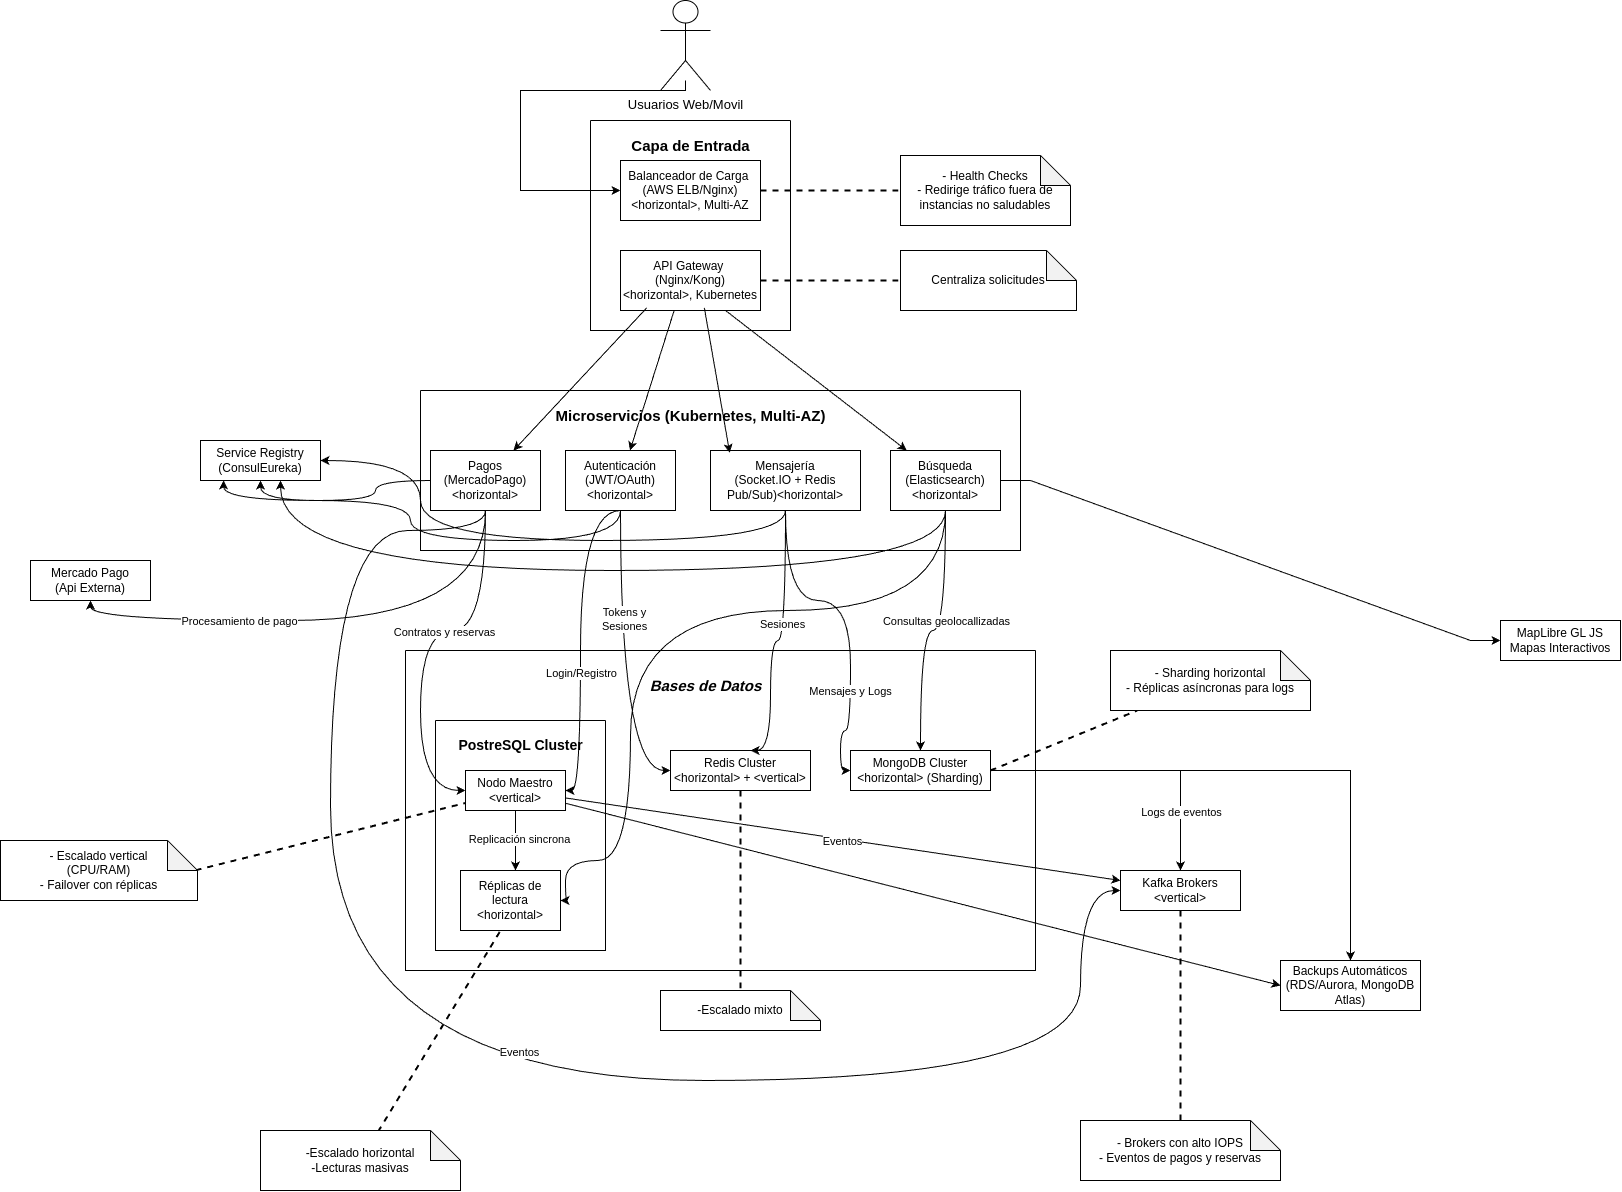
\includegraphics[width=\textwidth]{figures/diagrams/Diagrama de escalabilidad.png}
		\caption{Diagrama de escalabilidad del sistema CasaFácil}
	\end{figure}
	
	\textbf{Descripción del flujo:}
	\begin{itemize}
		\item Usuarios → balanceador → API Gateway → microservicios.
		\item Microservicios → DBs (PostgreSQL, MongoDB), Redis, Kafka.
		\item Servicio de pagos conecta a MercadoPago.
		\item Servicio de búsqueda consulta mapas externos (MapLibre).
		\item Registro de servicios facilita descubrimiento entre microservicios.
		\item Backups garantizan persistencia de datos.
	\end{itemize}
	
	\newpage
	\textbf{Alta disponibilidad y failover:}
	\begin{itemize}
		\item Balanceador redirige tráfico a instancias saludables.
		\item Kubernetes reinicia pods fallidos automáticamente.
		\item PostgreSQL con réplicas síncronas.
		\item MongoDB con réplicas asíncronas.
		\item Redis en cluster.
		\item Backups automáticos ante fallos catastróficos.
	\end{itemize}
	
	\textbf{Crecimiento ante demanda:}
	\begin{itemize}
		\item API Gateway y balanceador escalan horizontalmente.
		\item Kubernetes lanza más pods.
		\item PostgreSQL añade réplicas o CPU.
		\item MongoDB shardea nuevas colecciones.
		\item Redis escala en RAM/nodos.
		\item Kafka usa brokers más potentes.
	\end{itemize}
